\subsubsection*{CHIRPS e IMERG: comparación del apartado 2.1}
\subsubsection*{CHIRPS: los mismos diagramas y criterios}
Debajo de IMERG se presentan CHIRPS--lluvia local, lluvia local--caudal y CHIRPS--caudal, con idénticas unidades y colores por mes calendario. La gráfica lluvia local--caudal se repite para conservar la estructura de tres paneles: sus datos son exactamente los mismos y no constituyen un resultado independiente. CHIRPS es precipitación espacial promediada sobre la cuenca, no una estación terrestre. La comparación CHIRPS--IMERG usa exclusivamente los mismos 14 meses completos frente a Zaragoza y los mismos 285 meses completos frente a Q/R (1998--2022). No se compara el registro CHIRPS de 485 meses con el registro IMERG de 285 para decidir qué producto se ajusta mejor.
\subsubsection*{Dirección, forma, dispersión y puntos influyentes en CHIRPS}
CHIRPS--lluvia local y CHIRPS--Q muestran asociación positiva. La primera nube es relativamente alineada en esta muestra pequeña, aunque todos los acumulados CHIRPS están por encima de la lluvia local (debajo de 1:1 con la orientación elegida). CHIRPS--Q tiene una nube amplia; a lluvias similares corresponden caudales diferentes y no hay una relación determinista. Los colores se solapan, sin agrupamientos separados que permitan identificar regímenes por sí solos. En ambas fuentes, los caudales altos amplían la dispersión y noviembre de 2010 debe examinarse como valor influyente. La tabla de retirar-un-mes cuantifica la sensibilidad para cada relación; se conservan todos los valores originales.
\subsubsection*{¿Cuál tiene menor error frente a Zaragoza?}
En los mismos 14 meses, CHIRPS tiene sesgo +86,74, MAE 86,74 y RMSE 104,14 mm/mes; IMERG tiene sesgo +109,80, MAE 109,80 y RMSE 119,61 mm/mes. CHIRPS muestra menor discrepancia con la referencia puntual en esta muestra: su RMSE es aproximadamente 12,9 \% menor y su MAE 21,0 \% menor. Ambos sobreestiman todos los acumulados locales seleccionados. La relación CHIRPS--local es algo más fuerte (Pearson 0,82; Spearman 0,75) que IMERG--local (0,79; 0,71), pero la correlación no mide concordancia ni demuestra mayor exactitud en toda la cuenca. Zaragoza es una referencia puntual de cobertura corta; no basta para declarar un producto superior en general.
\begin{center}\small\begin{tabular}{lrrrrr}\hline
Fuente & n & Sesgo & MAE & RMSE & SD error \\ \hline
IMERG & 14 & 109,80 & 109,80 & 119,61 & 49,22 \\
CHIRPS & 14 & 86,74 & 86,74 & 104,14 & 59,80 \\
\hline\end{tabular}\end{center}
\subsubsection*{¿Cuál es más disperso? Depende de la comparación}
La dispersión se cuantifica con unidades y muestras iguales. Frente a la recta 1:1 con Zaragoza, la desviación estándar muestral del error P-local es 59,80 mm/mes para CHIRPS y 49,22 para IMERG: los errores CHIRPS son más variables aunque su sesgo y RMSE totales son menores. Alrededor de la recta lineal ajustada a lluvia local, el RMSE residual es 33,59 mm/mes para CHIRPS y 35,87 para IMERG: la nube CHIRPS es algo más estrecha alrededor de su propia recta. Frente a caudal, el RMSE residual en los mismos 285 meses es 58,89 m$^3$/s para CHIRPS y 56,85 para IMERG: IMERG tiene aproximadamente 3,5 \% menos dispersión residual y una asociación algo mayor. Estas rectas son resúmenes descriptivos calculados con todos los pares, no modelos validados ni errores de pronóstico.
\begin{center}\small\begin{tabular}{lrrrr}\hline
Fuente & Referencia & n & RMSE residual & Mediana abs. \\ \hline
IMERG & lluvia local & 14 & 35,87 & 14,86 \\
IMERG & caudal Q & 285 & 56,85 & 35,49 \\
IMERG & escorrentía R & 285 & 53,58 & 32,64 \\
CHIRPS & lluvia local & 14 & 33,59 & 25,80 \\
CHIRPS & caudal Q & 285 & 58,89 & 33,70 \\
CHIRPS & escorrentía R & 285 & 55,60 & 31,76 \\
\hline\end{tabular}\end{center}
\subsubsection*{Anomalías, rezagos y apoyo con escorrentía para CHIRPS}
Se resta la climatología de cada mes calendario construida con los mismos 285 meses de 1998--2022 para CHIRPS, IMERG, Q y R. CHIRPS--Q pasa de Pearson 0,58 y Spearman 0,60 en valores originales a 0,54 y 0,54 en anomalías. IMERG--Q pasa de 0,62 y 0,63 a 0,64 y 0,60. La asociación persiste para ambas fuentes; IMERG es más fuerte en anomalías dentro de este periodo común. Se exploran P(t-k) frente a Q(t)/R(t), con k=0--3 meses, preservando el calendario y excluyendo cada par inválido. La tabla permite contrastar los rezagos sin introducir lluvia futura. R se expresa en mm/mes y deriva de Q, por lo que no constituye evidencia independiente. Para las dos parejas con lluvia local permanece la limitación: los 14 meses no sustentan una climatología local de doce meses adecuada. Para CHIRPS, en original, el mayor Pearson explorado está en k=1 (0,60; n=274). No es una estimación causal del tiempo de respuesta. Para IMERG, en original, el mayor Pearson explorado está en k=0 (0,62; n=285). No es una estimación causal del tiempo de respuesta. Para CHIRPS, en anomalía, el mayor Pearson explorado está en k=0 (0,54; n=285). No es una estimación causal del tiempo de respuesta. Para IMERG, en anomalía, el mayor Pearson explorado está en k=0 (0,64; n=285). No es una estimación causal del tiempo de respuesta.
\begin{figure}[H]\centering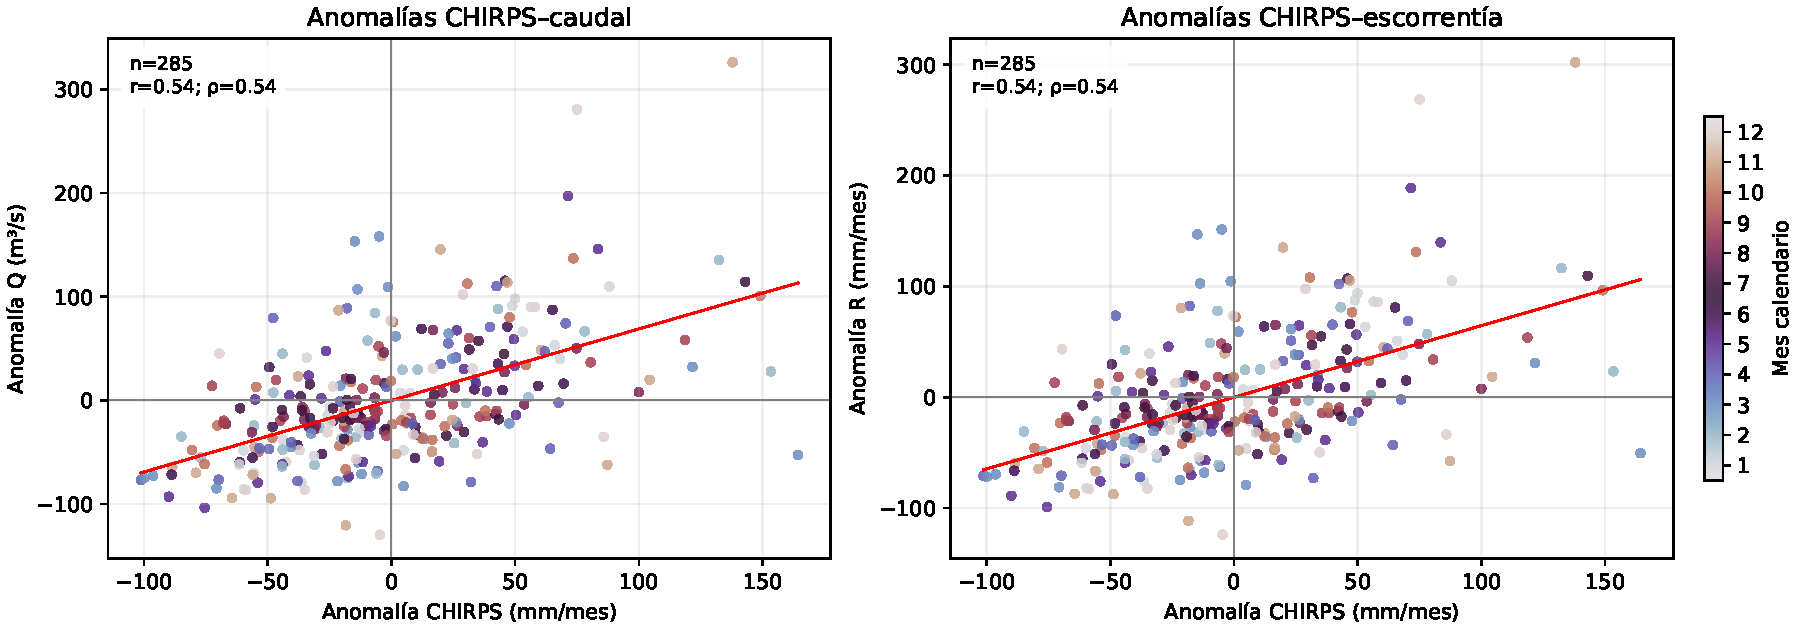
\includegraphics[width=\linewidth]{../apartado_2_1/anomalias_CHIRPS_21.pdf}\caption{Anomalías CHIRPS con climatología común 1998--2022.}\end{figure}
\begin{figure}[H]\centering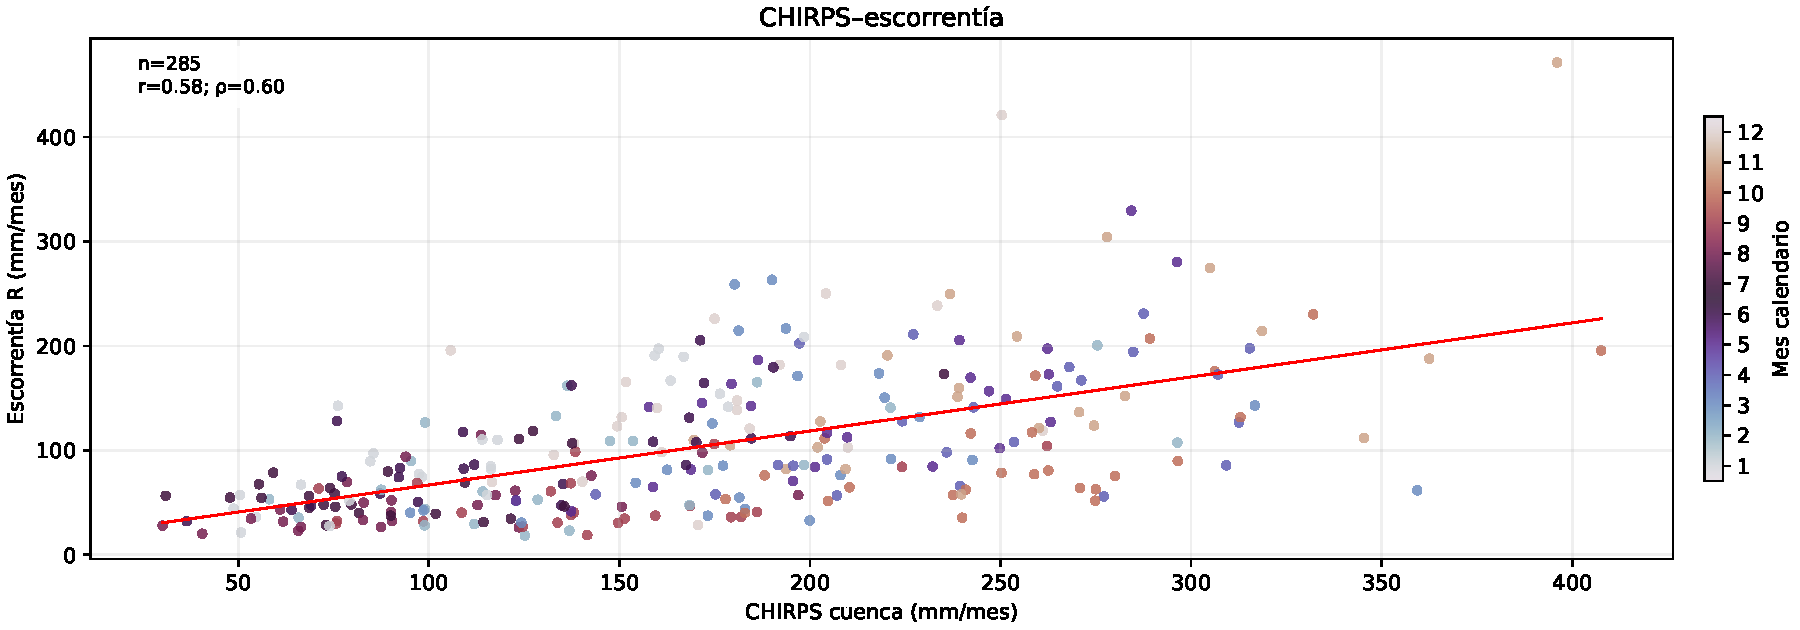
\includegraphics[width=\linewidth]{../apartado_2_1/laminas_CHIRPS_21.pdf}\caption{Apoyo con escorrentía mensual en láminas.}\end{figure}
\subsubsection*{Conclusión comparativa del 2.1}
CHIRPS se acerca más a Zaragoza en error medio y RMSE durante los 14 meses completos disponibles; IMERG se asocia algo más con el caudal y presenta menos dispersión alrededor de la recta P--Q en los 285 meses comunes, incluso después de retirar el ciclo anual. No hay un único ganador para todas las preguntas: error frente a lluvia local, variabilidad del error y asociación con caudal son criterios distintos. Ninguno de estos resultados demuestra causalidad ni una ventaja predictiva fuera de muestra. La comparación de anomalías locales requiere ampliar los registros completos de estaciones.
\subsubsection*{Correlaciones originales y anomalías: muestras comunes}
\begin{center}\small\begin{tabular}{lrrrrr}\hline
Fuente & Referencia & Serie & n & Pearson & Spearman \\ \hline
IMERG & lluvia local & original & 14 & 0,79 & 0,71 \\
IMERG & caudal Q & original & 285 & 0,62 & 0,63 \\
IMERG & caudal Q & anomalía & 285 & 0,64 & 0,60 \\
IMERG & escorrentía R & original & 285 & 0,62 & 0,63 \\
IMERG & escorrentía R & anomalía & 285 & 0,63 & 0,60 \\
CHIRPS & lluvia local & original & 14 & 0,82 & 0,75 \\
CHIRPS & caudal Q & original & 285 & 0,58 & 0,60 \\
CHIRPS & caudal Q & anomalía & 285 & 0,54 & 0,54 \\
CHIRPS & escorrentía R & original & 285 & 0,58 & 0,60 \\
CHIRPS & escorrentía R & anomalía & 285 & 0,54 & 0,54 \\
\hline\end{tabular}\end{center}
\subsubsection*{Sensibilidad CHIRPS: retirar un mes}
\begin{center}\small\begin{tabular}{lrrrr}\hline
Relación & Mes & r sin mes & r mínimo & r máximo \\ \hline
CHIRPS--lluvia local & 2018-09 & 0,87 & 0,78 & 0,87 \\
CHIRPS--caudal Q & 2010-11 & 0,56 & 0,56 & 0,59 \\
CHIRPS--escorrentía R & 2010-11 & 0,56 & 0,56 & 0,59 \\
\hline\end{tabular}\end{center}
\subsubsection*{Rezagos CHIRPS: calendario continuo}
\textbf{original.}\begin{center}\small\begin{tabular}{lrrrr}\hline
Referencia & k & n & Pearson & Spearman \\ \hline
caudal Q & 0,00 & 285 & 0,58 & 0,60 \\
caudal Q & 1,00 & 274 & 0,60 & 0,66 \\
caudal Q & 2,00 & 270 & 0,26 & 0,32 \\
caudal Q & 3,00 & 267 & -0,06 & -0,06 \\
escorrentía R & 0,00 & 285 & 0,58 & 0,60 \\
escorrentía R & 1,00 & 274 & 0,60 & 0,66 \\
escorrentía R & 2,00 & 270 & 0,27 & 0,32 \\
escorrentía R & 3,00 & 267 & -0,06 & -0,07 \\
\hline\end{tabular}\end{center}
\textbf{anomalía.}\begin{center}\small\begin{tabular}{lrrrr}\hline
Referencia & k & n & Pearson & Spearman \\ \hline
caudal Q & 0,00 & 285 & 0,54 & 0,54 \\
caudal Q & 1,00 & 274 & 0,41 & 0,42 \\
caudal Q & 2,00 & 270 & 0,30 & 0,36 \\
caudal Q & 3,00 & 267 & 0,30 & 0,35 \\
escorrentía R & 0,00 & 285 & 0,54 & 0,54 \\
escorrentía R & 1,00 & 274 & 0,41 & 0,42 \\
escorrentía R & 2,00 & 270 & 0,30 & 0,36 \\
escorrentía R & 3,00 & 267 & 0,30 & 0,35 \\
\hline\end{tabular}\end{center}
